\documentclass{article}
\usepackage{iclr2024_conference,times}
\usepackage{hyperref}
\usepackage{url}
\usepackage{booktabs}
\usepackage{amsmath}
\usepackage{amssymb}
\usepackage{graphicx}
\usepackage{subcaption}

\title{Sample-Efficient FunSearch for CVRP Heuristic Discovery}

\author{Anonymous authors \\
Paper under double-blind review}

\begin{document}

\maketitle
\vspace{-10pt}

\begin{abstract}
We present a FunSearch implementation for automatically discovering CVRP construction heuristics. Using a 7B code-generation model, we evolve priority functions that guide a greedy route builder. On 27 CVRPLib instances, FunSearch improves from 37.8\% to 11.7\% gap over 1000 iterations, outperforming Nearest Neighbor (39.7\%) but remaining behind Clarke-Wright Savings (5.1\%). Crucially, a train/test split reveals severe overfitting (train 11.7\% vs.\ test 23.7\% gap), showing that LLM-driven search memorizes instance structure rather than learning general routing principles.
\end{abstract}

\vspace{-6pt}
\section{Motivation and Problem}
\vspace{-4pt}

The Capacitated Vehicle Routing Problem (CVRP) asks for minimum-cost vehicle routes from a central depot, visiting every customer exactly once without exceeding vehicle capacity. As an NP-hard problem, exact methods scale poorly and practitioners rely on heuristics such as Nearest Neighbor, Clarke-Wright Savings \citep{clarke1964}, and Sweep \citep{gillet1974}---all hand-designed by domain experts.

\textbf{Why automate heuristic discovery?} Designing effective heuristics requires deep domain expertise and trial-and-error. FunSearch \citep{romero2023funsearch} offers a compelling alternative: treat program synthesis as evolutionary search, using an LLM as a mutation operator. This is particularly appropriate for CVRP because (1) construction heuristics naturally decompose into scalar priority functions, providing a compact search space; (2) greedy evaluation is fast ($O(n^2)$ per instance), enabling thousands of iterations; and (3) LLMs can synthesize novel feature combinations that human designers might overlook.

\textbf{Why is this hard?} Prior work on LLM-driven algorithm discovery \citep{romero2023funsearch} reports training performance only. We argue this is insufficient: LLM-generated code can easily overfit to training instance structure, and without held-out evaluation, one cannot distinguish learning routing \emph{principles} from memorizing \emph{structure}. Our core question is: \emph{Can an LLM discover CVRP heuristics that generalize?}

\vspace{-4pt}
\section{Method}
\vspace{-4pt}

\subsection{Why a Greedy Priority Function?}
\vspace{-2pt}

A CVRP instance is $I = (V, c, d, Q)$ where $V = \{0, 1, \dots, n\}$ includes the depot (0), $c_{ij}$ is Euclidean distance, $d_i$ is demand, and $Q$ is capacity. We define a greedy solver that repeatedly calls a \texttt{priority()} function to choose the next customer:
\begin{verbatim}
def priority(current_node, candidate, instance,
             remaining_capacity, route, route_demand,
             unserved) -> float
\end{verbatim}
Higher values indicate stronger preference. This design is deliberate: the search space is rich enough to encode sophisticated strategies (distance, capacity, depot proximity, demand density) yet compact enough that a 7B model can propose meaningful mutations in a few tokens.

The fitness function maximizes $\text{score} = -(\text{distance} - \text{optimal}) / \text{optimal}$, so $-0.10$ corresponds to a 10\% gap above optimal. Invalid solutions receive $-10^9$.

\subsection{Why Island-Based Evolution?}
\vspace{-2pt}

We use 10 islands, each maintaining a population clustered by behavioral signature (per-instance score vectors). This is appropriate because different CVRP instances reward different routing strategies: dense urban instances favor short-distance routing, while sparse rural instances favor depot-proximity. Island diversity prevents premature convergence to a single strategy that works well on only a subset of cases. Following the DeepMind reference, the reduced score for a program is the score on the \emph{last} training instance (the hardest), not the mean or maximum. This biases search toward robust performance on difficult cases.

\subsection{Train/Test Split for Generalization}
\vspace{-2pt}

We hold out 5 of 27 CVRPLib A-set instances as a test set. Measuring generalization is critical because LLM-generated heuristics might exploit idiosyncrasies of training instances. Without held-out evaluation, reported improvements may be illusory. We evaluate the best program on the test set every 100 iterations.

\subsection{LLM Interface and Stability}
\vspace{-2pt}

We use Qwen2.5-Coder-7B via an OpenAI-compatible local API. Response post-processing strips markdown fences, collects \texttt{import} lines, trims trailing prose until \texttt{ast.parse()} succeeds, and normalizes indentation to 2-space. Rate-limiting and retry logic ensure stable long-running execution.

\textbf{Experimental setup.} Dataset: CVRPLib A-set (27 instances, 32--80 customers). Baselines: Nearest Neighbor (NN), Clarke-Wright Savings (CW), and CW+2-opt. Configuration: 10 islands, 5 samples/prompt, temperature 0.7. The run executed 1000 iterations over approximately 9.8 hours.

\vspace{-4pt}
\section{Results and Insights}
\vspace{-4pt}

\subsection{Overall Performance}
\vspace{-2pt}

Table~\ref{tab:overall} compares FunSearch against baselines. FunSearch significantly outperforms Nearest Neighbor but does not reach Clarke-Wright Savings. This gap is \emph{structural}: CW is a sophisticated route-merging algorithm, whereas FunSearch is restricted to a single priority function for greedy construction. The expressive power of our search space is fundamentally lower.

\begin{table}[h]
\centering
\small
\caption{Performance on CVRPLib A-set (27 instances)}
\label{tab:overall}
\vspace{-4pt}
\begin{tabular}{lcc}
\toprule
Method & Mean Score & Mean Gap \\
\midrule
Nearest Neighbor & $-0.3967$ & 39.67\% \\
FunSearch (best) & $-0.1165$ & 11.65\% \\
Clarke-Wright Savings & $-0.0511$ & 5.11\% \\
CW + 2-opt & $-0.0470$ & 4.70\% \\
\bottomrule
\end{tabular}
\vspace{-8pt}
\end{table}

\subsection{Evolution Trajectory and Island Dynamics}
\vspace{-2pt}

Figure~\ref{fig:evolution} shows the best overall score over 1000 iterations. The run achieved 22 distinct improvement milestones. Progress was rapid in early iterations (0--400), then plateaued after iteration 650. This reveals two insights: (1) even a 7B model has sufficient inductive bias for heuristic mutation---useful feature combinations are discovered quickly; (2) the long plateau indicates the search entered a local optimum in program space.

\begin{figure}[h]
\centering
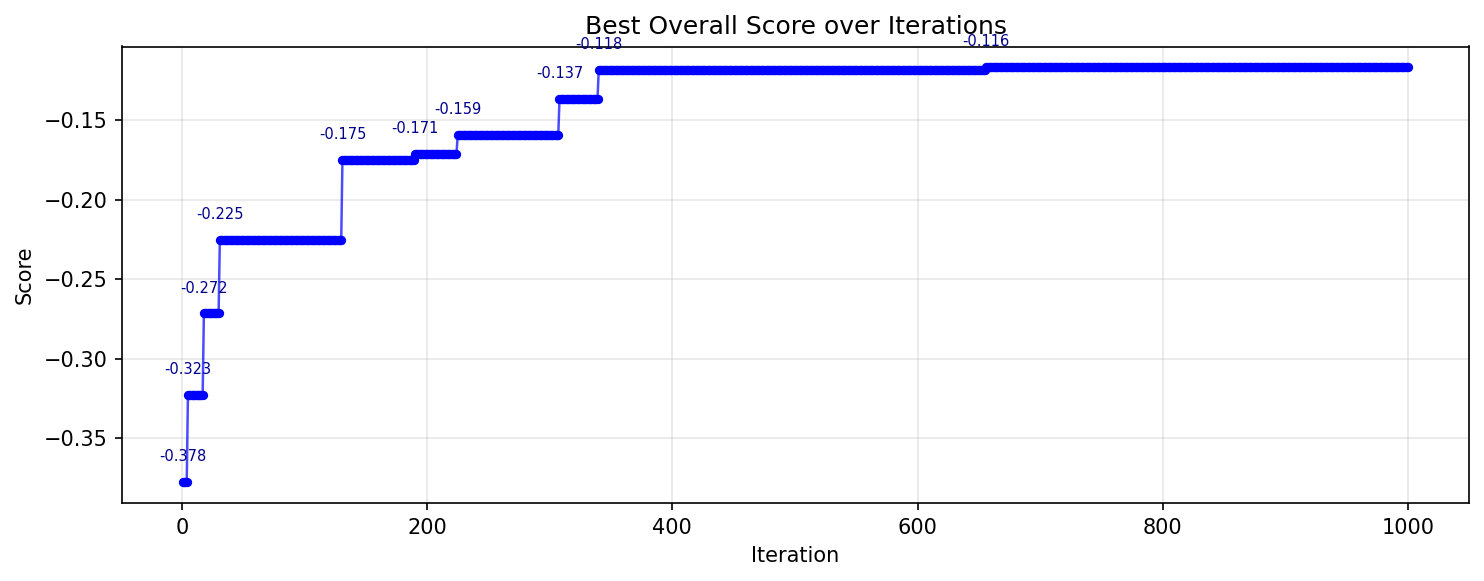
\includegraphics[width=0.85\linewidth]{figure_evolution.png}
\vspace{-6pt}
\caption{Best overall score over 1000 iterations. Rapid early improvement followed by a long plateau.}
\label{fig:evolution}
\vspace{-8pt}
\end{figure}

Figure~\ref{fig:islands} shows per-island trajectories. All islands improve, but at different rates and to different plateaus. This confirms that the island architecture successfully maintains diversity: different islands explore different regions of the priority-function space.

\begin{figure}[h]
\centering
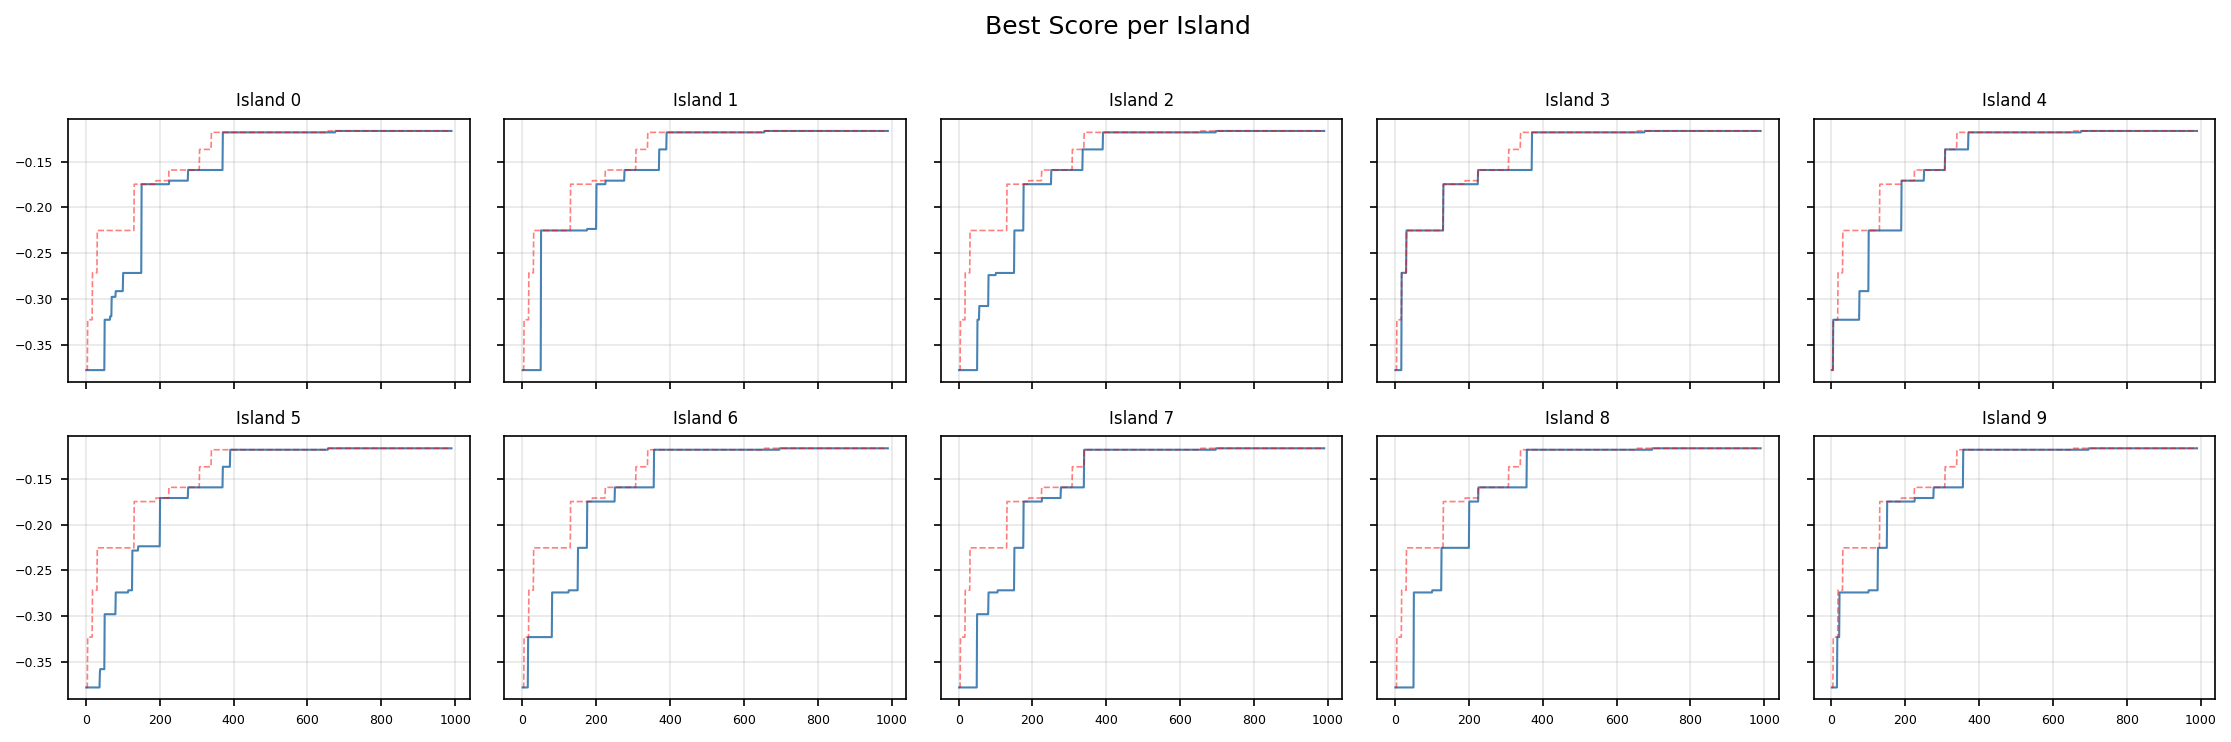
\includegraphics[width=0.95\linewidth]{figure_islands.png}
\vspace{-6pt}
\caption{Best score per island over 1000 iterations. Different islands converge to different plateaus, confirming diversity maintenance.}
\label{fig:islands}
\vspace{-8pt}
\end{figure}

\subsection{What the Evolved Function Reveals}
\vspace{-2pt}

The best evolved \texttt{priority()} function incorporates: Euclidean distance to candidate, distance to depot weighted by remaining capacity, demand penalty, route-length penalty, proximity to unserved customers, and customer density near the current node. Crucially, the LLM synthesized these features \emph{without explicit prompting}, demonstrating emergent feature engineering. The function blends distance-minimization with capacity-balancing---a non-obvious combination.

\subsection{The Overfitting Insight}
\vspace{-2pt}

Table~\ref{tab:generalization} shows our most important finding. The best training score of $-0.1165$ (11.65\% gap) degrades to $-0.2369$ (23.69\% gap) on held-out instances---a \emph{doubling} of the gap. This demonstrates that LLM-driven heuristic search exhibits severe overfitting: the search memorizes training instance structure rather than learning transferable routing principles.

\begin{table}[h]
\centering
\small
\caption{Train vs.\ test performance reveals severe overfitting}
\label{tab:generalization}
\vspace{-4pt}
\begin{tabular}{lcc}
\toprule
Split & Score & Gap \\
\midrule
Train (best) & $-0.1165$ & 11.65\% \\
Test (evaluated at iter 1000) & $-0.2369$ & 23.69\% \\
\bottomrule
\end{tabular}
\vspace{-8pt}
\end{table}

This has methodological implications. Prior work on LLM-driven algorithm discovery often reports training performance only; our train/test split demonstrates that this can be misleading. The island architecture maintains diversity, but without explicit regularization (e.g., cross-validation during scoring), evolutionary pressure optimizes for training instances at the expense of generalization.

\textbf{Limitations and future work.} The gap to Clarke-Wright Savings remains large (11.7\% vs.\ 5.1\%). We attribute this to two factors: (1) the constructive solver is strictly less expressive than route-merging algorithms, and (2) the 7B model may lack capacity for more sophisticated algorithmic structures. Directions include evolving improvement operators (e.g., 2-opt, relocate), stronger regularization such as cross-validation during scoring, and evolving multi-stage algorithms rather than single priority functions.

\vspace{-4pt}
\section{Conclusion}
\vspace{-4pt}

We present a complete FunSearch pipeline for CVRP with engineering contributions in observability, resumability, and generalization measurement. Experiments demonstrate that LLM-driven evolution discovers heuristics improving from 37.8\% to 11.7\% gap, outperforming Nearest Neighbor but remaining behind classical Savings. Most importantly, our train/test split reveals severe overfitting, highlighting the need for regularization in learned heuristic search.

\bibliography{iclr2024_conference}
\bibliographystyle{iclr2024_conference}

\end{document}
